% This file was created with tikzplotlib v0.10.1.
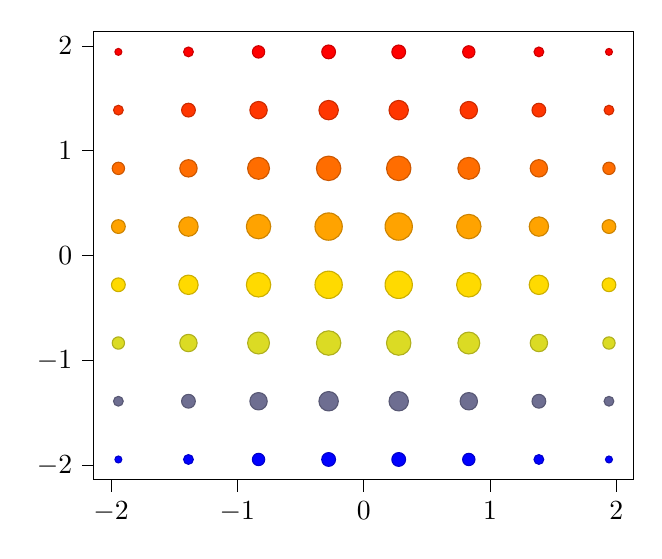
\begin{tikzpicture}

\definecolor{darkgray176}{RGB}{176,176,176}
\definecolor{steelblue31119180}{RGB}{31,119,180}

\begin{axis}[
tick align=outside,
tick pos=left,
x grid style={darkgray176},
xmin=-2.13620593547821, xmax=2.13620593547821,
xtick style={color=black},
y grid style={darkgray176},
ymin=-2.13620593547821, ymax=2.13620593547821,
ytick style={color=black}
]
\addplot [
  draw=steelblue31119180,
  fill=steelblue31119180,
  mark=*,
  only marks,
  scatter,
  scatter/@pre marker code/.append style={/tikz/mark size=\perpointmarksize},
  visualization depends on={\thisrow{sizedata} \as\perpointmarksize}
]
table{%
x  y  sizedata
-1.94200539588928 1.94200539588928 1.2521708
-1.38714671134949 1.94200539588928 1.7632555
-0.832288026809692 1.94200539588928 2.2239556
-0.277429342269897 1.94200539588928 2.4847505
0.277429342269897 1.94200539588928 2.4847505
0.832288026809692 1.94200539588928 2.2239556
1.38714671134949 1.94200539588928 1.7632555
1.94200539588928 1.94200539588928 1.2521708
-1.94200539588928 1.38714671134949 1.7632555
-1.38714671134949 1.38714671134949 2.4829438
-0.832288026809692 1.38714671134949 3.1316829
-0.277429342269897 1.38714671134949 3.4989233
0.277429342269897 1.38714671134949 3.4989233
0.832288026809692 1.38714671134949 3.1316829
1.38714671134949 1.38714671134949 2.4829438
1.94200539588928 1.38714671134949 1.7632555
-1.94200539588928 0.832288026809692 2.2239556
-1.38714671134949 0.832288026809692 3.1316829
-0.832288026809692 0.832288026809692 3.9499235
-0.277429342269897 0.832288026809692 4.413116
0.277429342269897 0.832288026809692 4.413116
0.832288026809692 0.832288026809692 3.9499235
1.38714671134949 0.832288026809692 3.1316829
1.94200539588928 0.832288026809692 2.2239556
-1.94200539588928 0.277429342269897 2.4847505
-1.38714671134949 0.277429342269897 3.4989233
-0.832288026809692 0.277429342269897 4.413116
-0.277429342269897 0.277429342269897 4.9306254
0.277429342269897 0.277429342269897 4.9306254
0.832288026809692 0.277429342269897 4.413116
1.38714671134949 0.277429342269897 3.4989233
1.94200539588928 0.277429342269897 2.4847505
-1.94200539588928 -0.277429342269897 2.4847505
-1.38714671134949 -0.277429342269897 3.4989233
-0.832288026809692 -0.277429342269897 4.413116
-0.277429342269897 -0.277429342269897 4.9306254
0.277429342269897 -0.277429342269897 4.9306254
0.832288026809692 -0.277429342269897 4.413116
1.38714671134949 -0.277429342269897 3.4989233
1.94200539588928 -0.277429342269897 2.4847505
-1.94200539588928 -0.832288026809692 2.2239556
-1.38714671134949 -0.832288026809692 3.1316829
-0.832288026809692 -0.832288026809692 3.9499235
-0.277429342269897 -0.832288026809692 4.413116
0.277429342269897 -0.832288026809692 4.413116
0.832288026809692 -0.832288026809692 3.9499235
1.38714671134949 -0.832288026809692 3.1316829
1.94200539588928 -0.832288026809692 2.2239556
-1.94200539588928 -1.38714671134949 1.7632555
-1.38714671134949 -1.38714671134949 2.4829438
-0.832288026809692 -1.38714671134949 3.1316829
-0.277429342269897 -1.38714671134949 3.4989233
0.277429342269897 -1.38714671134949 3.4989233
0.832288026809692 -1.38714671134949 3.1316829
1.38714671134949 -1.38714671134949 2.4829438
1.94200539588928 -1.38714671134949 1.7632555
-1.94200539588928 -1.94200539588928 1.2521708
-1.38714671134949 -1.94200539588928 1.7632555
-0.832288026809692 -1.94200539588928 2.2239556
-0.277429342269897 -1.94200539588928 2.4847505
0.277429342269897 -1.94200539588928 2.4847505
0.832288026809692 -1.94200539588928 2.2239556
1.38714671134949 -1.94200539588928 1.7632555
1.94200539588928 -1.94200539588928 1.2521708
};
\end{axis}

\end{tikzpicture}
